\documentclass[11pt,a4paper]{article}
\usepackage[margin=26mm]{geometry}
\usepackage[T1]{fontenc}
\usepackage[utf8]{inputenc}
\usepackage{lmodern,amsmath,amssymb,amsthm,mathtools,booktabs,graphicx,microtype}
\usepackage[colorlinks=true,linkcolor=blue!40!black,citecolor=blue!40!black,urlcolor=blue!40!black]{hyperref}
\usepackage{xcolor}
\usepackage[nameinlink,noabbrev]{cleveref}
\newtheorem{lemma}{Lemma}[section]
\theoremstyle{remark}
\newtheorem{remark}{Remark}[section]
\DeclareMathOperator{\supp}{supp}
\setlength{\emergencystretch}{3em}
\allowdisplaybreaks
\title{Certified finite-block influences\\for the square-lattice Ising model}
\author{Cambyse Rouz\'e \and Daniel Stilck Fran\c{c}a}
\date{Numerical supplement, version 1.0.0}
\begin{document}
\maketitle
\noindent This note documents the reproducibility package for
\emph{Rapid mixing of Gibbs samplers via quantum Dobrushin--Shlosman conditions}.
It records the finite-volume calculation and explicit constants used in the
Ising example. References to general quantum-dynamical constructions and
perturbation estimates refer to that companion manuscript.
\section{Certification of the Ising block example}
\label{app:ising-certification}

\subsection{Finite-block influences and numerical certificates}
\label{app:ising-blocks}

On the square torus with $L^2$ sites, consider
\begin{equation}
 H(g)=-J\sum_{\langle i,j\rangle}Z_iZ_j-g\sum_iX_i,
 \qquad x=\beta J.
 \label{qp:ising-model}
\end{equation}
At $g=0$, the exact single-site influence is
$c_{ij}=\frac12\tanh(2x)$, so the single-site certificate is
\begin{equation}
 \kappa(x,1)=1-2\tanh(2x).
 \label{qp:ising-singleton}
\end{equation}
It fails for $x\ge\frac12\operatorname{arctanh}(1/2)\simeq0.27465$.
We exhibit positive block certificates at $x=0.35$ and $x=0.36$ by
a finite computation, then apply the classical-reference perturbation theorem of the companion manuscript.

Take all $N$ translates of an $\ell\times\ell$ square, each with
rate $a_B=\ell^{-2}$, and assume $L\ge2\ell+2$.
Every site belongs to exactly $\ell^2$ blocks. Each block has
$4\ell$ distinct exterior neighbors. Write $c_p(x,\ell)$ for
$c_{Bj}$ when $j$ meets position $p$ along one side;
rotations identify the four sides and reflection gives
$c_p=c_{\ell+1-p}$.

\begin{lemma}[Exact influence from ferromagnetic monotonicity]
\label{qp:ising-influence}
Let $m_i^{\xi,\pm_j}$ be the magnetization at $i\in B$ with the
exterior spin $j$ fixed to $\pm1$ and the other exterior spins fixed
to $\xi$. For the ferromagnetic reference in \eqref{qp:ising-model},
\begin{equation}
 c_{Bj}=\frac12\max_\xi\sum_{i\in B}
       \bigl(m_i^{\xi,+_j}-m_i^{\xi,-_j}\bigr),
 \label{qp:ising-magnetizations}
\end{equation}
where the maximum ranges over the other $4\ell-1$ exterior neighbors.
\end{lemma}
\begin{proof}
Ferromagnetic monotonicity gives a coupling of the two conditional
Gibbs laws with $\sigma\ge\sigma'$ coordinatewise; it follows, for
example, by coupling their single-site heat baths with common uniform
random numbers and passing to stationarity. In this coupling the
Hamming distance is $\frac12\sum_{i\in B}(\sigma_i-\sigma'_i)$,
so its expectation gives the upper bound in
\eqref{qp:ising-magnetizations}. The function
$f(\sigma)=\frac12\sum_{i\in B}\sigma_i$ is $1$-Lipschitz for
Hamming distance, giving the reverse bound by Kantorovich duality.
Only exterior neighbors enter the conditional Hamiltonian.
\end{proof}

For a fixed site $j$, each side position occurs in four blocks
that have $j$ as an exterior neighbor. Thus the exact classical
and lifted margins coincide and equal
\begin{equation}
 \kappa(x,\ell)=1-\frac4{\ell^2}\sum_{p=1}^{\ell}c_p(x,\ell).
 \label{qp:ising-margin}
\end{equation}
We evaluate \eqref{qp:ising-magnetizations} by a column transfer
matrix with $2^\ell$ states, tracking the partition function and
the expected number of positive spins. The search exhausts all
boundary configurations, with global spin flip removing one binary
choice. Positive-arithmetic error bounds enclose every computed
$c_p$ within $10^{-9}$; Subsection~\ref{app:ising-computation}
gives the algorithm and certification details.

\begin{table}[htbp]
\centering
\begin{tabular}{c r r r r}
\toprule
$\ell$ & $x=0.30$ & $x=0.35$ & $x=0.40$ & $x=0.42$\\
\midrule
1 & -0.074099 & -0.208736 & -0.328074 & -0.371618 \\
2 & 0.035426 & -0.186278 & -0.417502 & -0.511628 \\
3 & 0.123728 & -0.170668 & -0.520613 & -0.675481 \\
4 & 0.229515 & -0.097434 & -0.533118 & -0.741202 \\
5 & 0.317415 & -0.026701 & -0.536402 & -0.798591 \\
6 & 0.391737 & 0.043216 & -0.525389 & -0.837924 \\
\midrule
First $\ell$ with $\kappa>0$ & 2 & 6 & $>6$ & $>6$\\
First $\ell$ with $\kappa\ge1/2$ & $>6$ & $>6$ & $>6$ & $>6$\\
\bottomrule
\end{tabular}
\caption{Square-block margins $\kappa(x,\ell)$, rounded to six
decimal places. Each unrounded value has certified error below
$4.1\times10^{-9}$. The last two rows refer to the search
$1\le\ell\le6$; $>6$ means that no tested size passed the stated test.}
\label{tab:ising-blocks}
\end{table}

\begin{figure}[htbp]
\centering
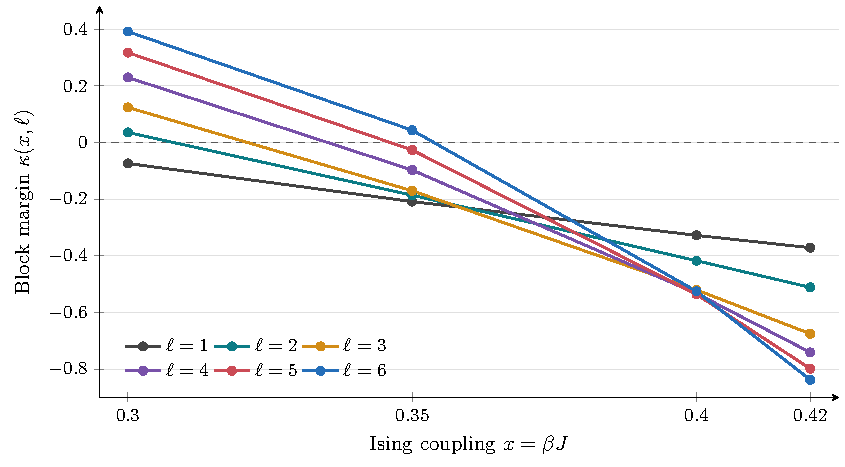
\includegraphics[width=.82\textwidth]{numerical/ising_blocks/ising_block_margins.pdf}
\caption{The certified margins in \Cref{tab:ising-blocks}.
Positive values give block certificates. Lines join the computed
points as visual guides.}
\label{fig:ising-blocks}
\end{figure}

In particular, $(x,\ell)=(0.35,6)$ has margin greater than $0.0432$.
One further size gives $\kappa(0.36,7)>0.0125$, whereas
\eqref{qp:ising-singleton} is negative at both temperatures.
For either pair choose the displayed lower bound as $\kappa$.
The finite block certificate is the hypothesis used in this
application. Strong mixing for squares \cite{MOS1994} and the
finite-volume DS tests approaching criticality \cite{Shlosman}
provide the broader classical context.

\subsection{Exhaustive boundary search and arithmetic bounds}
\label{app:ising-computation}

We describe the finite computation underlying \Cref{tab:ising-blocks}
and the two positive certificates in the Ising example of the companion manuscript.
The code, certified input weights, full coefficient tables, and
maximizing boundary configurations are supplied in
\texttt{numerical/ising\_blocks/}.

For a column $s\in\{-1,+1\}^{\ell}$, let $n_+(s)$ count its positive
spins. If $t_c,b_c$ are the top and bottom boundary spins at column
$c$, define
\[
 K(s,s')=e^{x\sum_{i=1}^{\ell}s_is'_i},\qquad
 V_c(s)=\exp\!\left[x\left(\sum_{i=1}^{\ell-1}s_is_{i+1}
                         +t_cs_1+b_cs_\ell\right)\right].
\]
Keep the entire left boundary $a$ as a matrix index. Initialize
$Z_1(a,s)=K(a,s)V_1(s)$ and $U_1(a,s)=n_+(s)Z_1(a,s)$, and iterate
\begin{align*}
 Z_{c+1}(a,s')&=V_{c+1}(s')\sum_sK(s,s')Z_c(a,s),\\
 U_{c+1}(a,s')&=V_{c+1}(s')\sum_sK(s,s')
                     [U_c(a,s)+n_+(s')Z_c(a,s)].
\end{align*}
Finally multiply each matrix by $K$ to incorporate every right
boundary $b$. The ratio $U(a,b)/Z(a,b)$ is the expected total number
of positive spins. Differences between left boundary rows differing
at position $p$ therefore give exactly the quantities maximized in
\eqref{qp:ising-magnetizations}. The matrix $K$ is a tensor product
of $\ell$ two-by-two matrices, so each transfer is evaluated by
successive two-component transforms.

Global spin flip preserves each response difference, allowing the
first top boundary spin to be fixed to $+1$. We enumerate all
$2^{2\ell-1}$ remaining top/bottom patterns, while the two matrix
indices cover all left/right patterns. For each $p$, this checks
all $2^{4\ell-2}$ representatives of the other exterior spins.
Reflection is used to check $c_p=c_{\ell+1-p}$, rather than to
restrict the maximizing boundary. At $(x,\ell)=(0.35,6)$ the three
inequivalent coefficients, each with error below $10^{-9}$, are
\[
 c_1=1.10740048984,\qquad c_2=1.52878638950,\qquad
 c_3=1.66933990243.
\]
They give $\kappa(0.35,6)>0.0432162700$.
The additional search at $(0.36,7)$ gives
$\kappa(0.36,7)>0.0125511558$.

Here is an arithmetic certificate for all entries used in the paper.
The input values $x$ are exact terminating decimals. The weights
$e^{kx}$, $|k|\le9$, are computed with a correctly rounded
100-digit decimal exponential; an enclosure of width $2\times10^{-98}$
certifies that each binary64 weight has relative error at most
$2^{-52}$. The search uses round-to-nearest binary64 arithmetic
without reassociation. Every entry of $Z$ and $U$ is assembled from
nonnegative sums and products. For $\ell\le8$, the number of
unit-roundoff factors along any operation path is at most
$4\ell^2+5\ell+5\le301$. With $\epsilon_{\rm fp}=2^{-53}$, the
conservative bound
\[
 \gamma=\frac{4096\epsilon_{\rm fp}}{1-4096\epsilon_{\rm fp}}
 <4.55\times10^{-13}
\]
therefore bounds the relative error of every positive $Z$ or $U$;
a zero $U$ is represented exactly. All positive intermediates lie
between $e^{-61}$ and $64\,2^{64}e^{61}$ for the parameters used,
so there is neither overflow nor underflow.

The ratio $U/Z$ lies in $[0,\ell^2]$. Its absolute error is at most
\[
 \ell^2\left[\frac{1+\gamma}{1-\gamma}
                       (1+\epsilon_{\rm fp})-1\right].
\]
Subtracting two such ratios gives error below $1.3\times10^{-10}$
for $\ell\le8$. Taking a maximum preserves this absolute-error
bound, so we enclose each $c_p$ by the computed maximum plus or
minus $10^{-9}$, with endpoints rounded outward. The corresponding
margin has error at most $4\times10^{-9}/\ell+10^{-13}$, including
the final summation. An independent enumeration of all interior
and exterior spin configurations for $\ell=1,2,3$ agrees with the
transfer computation to within $2\times10^{-13}$. It also verifies
\eqref{qp:ising-singleton}, zero influence at $x=0$, and the
small-coupling limit.

\subsection{Explicit shell constants for the square-lattice example}
\label{app:ising-shell-constants}

We give explicit perturbation windows for the block certificates in
Subsection~\ref{app:ising-blocks}. Rescale the Hamiltonian by $\beta$, so that
the inverse temperature is one, the edge norm is $x=\beta J$, and the
on-site perturbation norm is $u=\beta|g|\le u_0\le1$.
Let $B$ be an $\ell\times\ell$ square on a torus with $L\ge\ell+2$,
$R_B=B^{\le1}$, and $R_{B,r}=B^{\le r+1}$. Put
\begin{equation}
 b=\ell^2,\qquad r_0=\ell^2+4\ell,\qquad
 \chi=r_0/b,\qquad w=4\ell x,\qquad
 T=e^{4\ell x}\log\frac{32r_0\chi}{\kappa},
 \label{qp:ising-parameters}
\end{equation}
where $\kappa$ is the chosen certified lower bound on the block margin.
The on-site perturbation changes no crossing interaction, so
the local perturbation bound of the companion manuscript uses $E=e^w$.
The corresponding infinite-lattice neighborhood has cardinality
$\ell^2+4\ell(r+1)+2r(r+1)\le r_0(r+1)^2$.
Passing to the torus can only reduce this cardinality, and translation
invariance gives weighted overlap $|R_{B,r}|/b$. Thus
the polynomial-growth and weighted-overlap hypotheses of the companion manuscript holds with $D=2$, $V=r_0$, and $\Xi=\chi$.

An explicit real-time restriction bound is
\begin{equation}
 \|\tau_t^K(A)-\tau_t^{K'}(A)\|
 \le8|S|\|A\|\min\{1,(e^{v|t|}-1)e^{-q}\},
 \qquad v=32e x,
 \label{app:ising-explicit-lr}
\end{equation}
when $A$ is supported on $S$ and the smaller restriction contains
$S^{\le q}$. To verify the constants, remove all on-site terms in the
interaction picture. The remaining time-dependent edge interactions
still have norm at most $x$. More explicitly, for a fixed observable
$F$ define $C_F(S,t)=\sup_{A\in\mathcal B(S)}
\|[\tau_t^{K'}(A),F]\|/\|A\|$. The usual interaction-picture
commutator recurrence is bounded by
\[
 C_F(S,t)\le C_F(S,0)
       +2x\sum_{e:e\cap S\ne\varnothing}
              \int_0^{|t|}C_F(e,s)\,ds,
 \qquad
 C_F(S,0)\le2\|F\|\mathbf1_{S\cap\supp F\ne\varnothing}.
\]
Enlarging the edge sum to all edges meeting $S$ only increases it.
Its iteration is over consecutive overlapping edges, rather than
successively growing operator supports: there are at most $4|S|$
choices of the first edge and at most seven choices of each subsequent
edge overlapping its predecessor. Apply this bound with $F$ each
edge term crossing the restriction boundary in Duhamel's formula.
For $n$ interior edges, summing also over the final boundary edge
costs at most $4|S|7^n$, and only $n\ge q$ can reach that boundary.
The norm of the final edge is at most $x$ and its commutator contributes
a factor two. Integrating
$8x|S|\|A\|\sum_{n\ge q}(14xs)^n/n!$ over $0\le s\le|t|$ gives
\[
 \|\tau_t^K(A)-\tau_t^{K'}(A)\|
 \le\frac47 |S|\|A\|
       \sum_{n\ge q+1}\frac{(14x|t|)^n}{n!}
 \le\frac4{7e}|S|\|A\|e^{-q}(e^{14e x|t|}-1).
\]
Indeed, a chain reaching the boundary has at least $q$ interior edges
before the final Duhamel edge. The trivial bound $2\|A\|$ then proves
\eqref{app:ising-explicit-lr}. This argument also applies to weakened
crossing edges in the QBP interpolation and to a passive reference.

Set
\begin{equation}
 \bar v=\max\{1,32ex\},\qquad
 \mu=\frac1{2\bar v},\qquad C_{\rm tr}=36+4\bar v.
 \label{app:ising-transform-constants}
\end{equation}
The kernel representations imply, separately for
$\mathcal Q=\mathcal F$ and $\mathcal Q=\mathcal G$,
\begin{equation}
 \|\mathcal Q_K(A)-\mathcal Q_{K'}(A)\|
 \le C_{\rm tr}|S|\|A\|e^{-\mu q}.
 \label{app:ising-transform-bound}
\end{equation}
For completeness, split the time integrals at
$t_q=(q+1)/(2\bar v)$. The positive kernel satisfies
$\int_{|t|>t_q}p_1(t)\,dt\le e^{-2\pi t_q}$.
The short-time part of its integral is bounded by
$8e^{1/2}|S|\|A\|e^{-q/2}$, and its long-time part by
$2\|A\|e^{-\pi(q+1)/\bar v}$.
For the odd kernel, the short-time part is bounded by
\[
 \frac8\pi|S|\|A\|e^{-q}
 \int_0^{(q+1)/2}\frac{e^z-1}{z}\,dz
 \le\frac{8e^{1/2}}\pi|S|\|A\|e^{-q/2}.
\]
The long-time part is at most
\[
 \frac2\pi\|A\|\log\coth(\pi t_q)
 \le\frac4\pi(1+\bar v/\pi)\|A\|
          e^{-\pi(q+1)/\bar v}.
\]
Here we used $\log\coth z\le2e^{-2z}/(1-e^{-2z})$ and
$(1-e^{-a})^{-1}\le1+a^{-1}$. The choices in
\eqref{app:ising-transform-constants} dominate both bounds, including
$q=0$.

Define the following finite constants:
\begin{align}
 E&=e^w,\qquad P=2^{r_0},\qquad a_0=r_0/2,\qquad J_0=1+a_0u_0,\notag\\
 K_{\rm Q}&=E C_{\rm tr}r_0w,\qquad
 L_{\rm Q}=\max\{E,e^\mu K_{\rm Q}\},\notag\\
 K_{\rm P}&=4PJ_0C_{\rm tr}r_0,\qquad
 L_{\rm P}=\max\{Pa_0(2+a_0u_0)u_0,e^\mu K_{\rm P}\},\notag\\
 C_s&=(8r_0+34)(K_{\rm Q}+K_{\rm P})
       +2C_{\rm tr}r_0(L_{\rm Q}+L_{\rm P}).
 \label{app:ising-shell-constants-explicit}
\end{align}
Then the augmented physical generators satisfy
\begin{equation}
 \|\mathcal A_{B,R_{B,r+1}}(H)-\mathcal A_{B,R_{B,r}}(H)\|_\diamond
 \le C_s(r+1)^3e^{-\mu r}.
 \label{app:ising-certified-shell}
\end{equation}
To check this propagation, the dressing and its inverse have norms at
most $e^{w/4}$. Equation~\eqref{app:ising-transform-bound} and variation
of constants bound each successive dressing difference by
$e^{w/4}(C_{\rm tr}r_0w/4)e^{-\mu r}$.
Telescoping its four conjugating factors bounds the successive QBP
jump-map and loss differences by $K_{\rm Q}e^{-\mu r}$.
For pinching, each jump has norm at most $J_0$ and successive difference
at most $2C_{\rm tr}r_0e^{-\mu r}$. Summing over the $P$ projectors
therefore bounds the jump-map and loss differences by
$K_{\rm P}e^{-\mu r}$.

For either part of the loss, write $A_m=S_m-S_{m-1}$ for $m\ge1$,
with $A_0=S_0$ for QBP and $A_0=S_0-I$ for pinching.
The corresponding constants above give
$\|A_m\|\le L e^{-\mu m}$ and
$\|S_{r+1}-S_r\|\le K e^{-\mu r}$.
The coherent shell is
\[
 \mathcal G_{H_{R_{B,r+1}}}(A_{r+1})
 +\sum_{m=0}^r
 [\mathcal G_{H_{R_{B,r+1}}}-\mathcal G_{H_{R_{B,r}}}](A_m).
\]
The smaller region contains the $(r-m)$-neighborhood of the support
$R_{B,m}$; thus the distance in the $m$th term is exactly $q=r-m$,
with no shell offset. The multiplier bound in the coherent-multiplier lemma of the companion manuscript
and \eqref{app:ising-transform-bound} give respectively
\[
 (r_0+4)K(r+2)^2e^{-\mu r},\qquad
 C_{\rm tr}r_0L\sum_{m=0}^r(m+1)^2e^{-\mu r}.
\]
Their sum is at most
$[4(r_0+4)K+C_{\rm tr}r_0L](r+1)^3e^{-\mu r}$.
Adding the jump-map and anticommutator differences, and twice the
coherent difference, proves \eqref{app:ising-certified-shell} with
\eqref{app:ising-shell-constants-explicit}.

The infinite tail needed in the perturbation-threshold formula of the companion manuscript is bounded
without numerical truncation. For $R+2\ge14/\mu$,
\begin{equation}
 \sum_{r\ge R}(r+2)^7e^{-\mu r}
 \le\frac{(R+2)^7e^{-\mu R}}{1-e^{-\mu/2}},
 \label{app:ising-tail-majorant}
\end{equation}
because the ratio of successive summands is at most $e^{-\mu/2}$.
Use $V=r_0$, $\Xi=\chi$, $C_{\rm loc}$ from
the local-continuity formula of the companion manuscript with $E=e^w$, and the constants above in
the aggregate perturbation-error formula of the companion manuscript. Choose $R_*$ so the majorant multiplied by $B_0$
is at most $\kappa/8$, and choose
$u_*\le\min\{u_0,\kappa/[8A(1+R_*)^8]\}$.
The supplied script \texttt{numerical/ising\_blocks/perturbation\_window.py}
performs this calculation using outward-rounded decimal arithmetic.
With $u_0=1$, it gives the sufficient choices
\[
 \begin{array}{c|c|c|c|c|c}
  x&\ell&\kappa&T\text{ (approximately)}&R_*&u_*\\\hline
  0.35&6&0.0432&4.9864\times10^4&9481&10^{-68}\\
  0.36&7&0.0125&3.0169\times10^5&10800&10^{-76}
 \end{array}
\]
The margins in this table are certified lower bounds supplied by the
separate finite-volume computation. These small sufficient windows
reflect the conservative continuity and shell constants.

\begin{remark}[The boundary cost of two-dimensional blocks]
For these squares, $w=4\ell x$ grows with the perimeter and the
guaranteed interior erasure rate is $e^{-4\ell x}$. Thus larger
blocks improve the classical certificate at the cost of a longer
internal time and a smaller sufficient perturbation window.
In one dimension the boundary has bounded size independently of
the block length. The windows here establish existence; we expect
the admissible range of $|\beta g|$ at these fixed temperatures
to be of order one.
\end{remark}

\begin{thebibliography}{2}
\bibitem{MOS1994} F.~Martinelli, E.~Olivieri, and R.~H.~Schonmann.
For 2-D lattice spin systems weak mixing implies strong mixing.
\emph{Communications in Mathematical Physics} \textbf{165}, 33--47 (1994).
\href{https://doi.org/10.1007/BF02099735}{doi:10.1007/BF02099735}.
\bibitem{Shlosman} S.~B.~Shlosman.
The critical temperature $T_{cr}(\mathrm{Ising})$ is DS-computable (2025).
\href{https://arxiv.org/abs/2505.24750v2}{arXiv:2505.24750v2}.
\end{thebibliography}
\end{document}
